\documentclass[conference,letterpaper]{IEEEtran}

\usepackage{amsmath,amssymb,amsfonts}
% The current IEEE guide writes out each citation number instead of ranges.
\usepackage[nocompress]{cite}
\bibliographystyle{IEEEtran}
\usepackage[utf8]{inputenc}
\usepackage[T1]{fontenc}
\usepackage{graphicx}
% Caption the in-text wide displays without replacing IEEE captions.
\usepackage{capt-of}
\usepackage[nospread]{cuted}
\usepackage{float}
\usepackage{booktabs}
\usepackage{multirow}
\usepackage{array}
\usepackage{microtype}
\usepackage[bottom]{footmisc}
\usepackage[hidelinks]{hyperref}

\newcommand{\best}[1]{\textbf{#1}}
\newcommand{\second}[1]{\underline{#1}}
\newcommand{\sg}{\operatorname{sg}}

\title{Efficient JPEG Restoration in the Wavelet Domain via Mean Flows}

\author{%
\IEEEauthorblockN{\c{S}tefan-Alexandru Asandei}
\IEEEauthorblockA{Independent Researcher\\
asandei.stefanel@gmail.com}
\and
\IEEEauthorblockN{Mihai-Alexandru Radu}
\IEEEauthorblockA{Faculty of Physics\\
``Alexandru Ioan Cuza'' University of Ia\c{s}i\\
mihai.radu@student.uaic.ro}
}

\begin{document}
% List all authors up to six, then the first author followed by et al.
\bstctlcite{IEEEreferenceControl}
% Avoid stretching short text fragments around in-text wide tables.
\raggedbottom
\maketitle

\begin{abstract}
Latest JPEG restoration systems achieve strong quality with large models, yet often remain too slow and expensive for efficient on-device deployment.  We present a 65M-parameter generative restorer that attains the lowest LPIPS among the compared settings at QF 10 and 20 on LIVE-1, Urban100, and DIV2K-val while sustaining 8.05 images/s at $1024\times1024$ on a single RTX 3090.  Trained from scratch, the model replaces the learned VAE encoder-decoder with an exactly invertible two-level Haar transform, predicts a clean wavelet-domain residual through a rank-enhanced linear-attention DiT that estimates compression severity internally, and is optimized with an improved MeanFlow objective that enables inference in one or two network evaluations without distillation.  Large pretrained priors remain stronger under severe compression (QF 5), whereas our model prioritizes throughput for deployment-constrained restoration.
\end{abstract}

\section{Introduction}

JPEG compression removes high-frequency information and introduces blocking, ringing, and color discontinuities~\cite{wallace1991jpeg}. Feed-forward restorers often over-smooth, whereas DiffBIR, SUPIR, and SODiff reuse large pretrained diffusion priors~\cite{lin2024diffbir,yu2024supir,yang2025sodiff}. Even one-step latent restoration retains the cost of a large denoiser, VAE encoding and decoding, and semantic conditioning.

\begin{figure}[H]
\centering
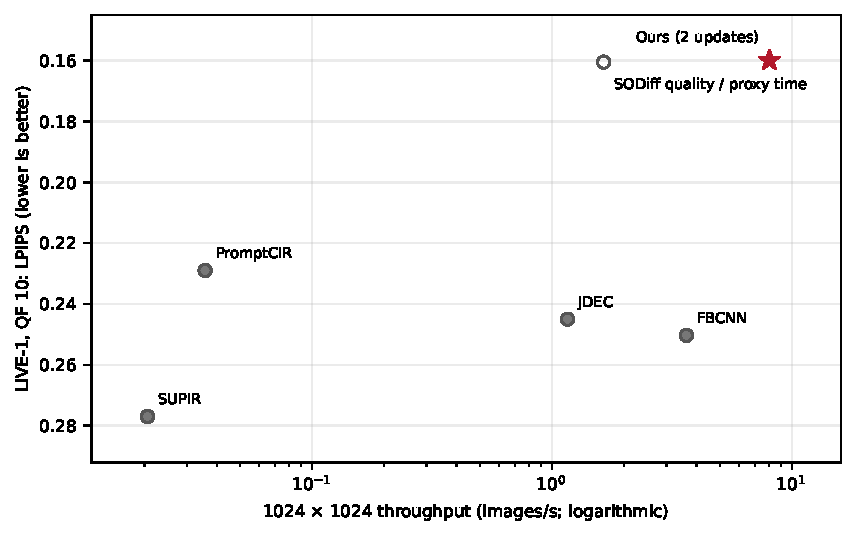
\includegraphics[width=\linewidth]{figures/pdf/pareto_quality_vs_throughput.pdf}
\caption{LIVE-1 QF 10 quality versus $1024^2$ throughput. The hollow point pairs published SODiff quality with an SD 2.1 timing proxy, not a measured SODiff system. Other points use local measurements; inference settings remain method-specific.}
\label{fig:pareto}
\end{figure}

We train a 65.32M-parameter restorer from scratch without a text encoder, pretrained generator, or VAE. A two-level Haar transform organizes clean-residual prediction~\cite{li2025jit,lu2026pixelmeanflow}, and an improved MeanFlow objective~\cite{geng2025meanflow,geng2025improved} enables one- or two-evaluation inference. The resulting quality-efficiency trade-off is strongest at QF 10 and 20; large pretrained priors remain stronger under severe compression and on several perceptual metrics.\footnote{Training, evaluation, and verification code: \url{https://github.com/stefanasandei/jpeg-restore}. Model weights: \url{https://huggingface.co/asandeistefan/jpeg-restore-meanflows}.}

Our contributions are:
\begin{itemize}
\item a compact, latent-free conditional MeanFlow formulation for JPEG restoration using clean residuals in a two-level Haar domain;
\item a SANA-style linear DiT integrating RELA and internal JPEG-severity estimation; and
\item a quality-efficiency study across three datasets, backbone resolution scaling, and complete restoration systems.
\end{itemize}

\section{Related Work}

FBCNN estimates compression severity and conditions a convolutional restorer on it~\cite{jiang2021fbcnn}; JDEC operates on JPEG coefficients~\cite{han2024jdec}; PromptCIR learns degradation prompts~\cite{li2024promptcir}. DiffBIR and SUPIR instead reuse pretrained generative priors~\cite{lin2024diffbir,yu2024supir}. SODiff specializes Stable Diffusion 2.1 to one-step JPEG restoration, retaining its UNet and VAE endpoints~\cite{yang2025sodiff,stable_diffusion_21}.

Rectified Flow learns an instantaneous transport velocity~\cite{liu2023rectifiedflow}, while MeanFlow learns interval-average velocity for few-update sampling~\cite{geng2025meanflow,geng2025improved}. We combine this objective with the clean-data prediction of JiT and pixel MeanFlow~\cite{li2025jit,lu2026pixelmeanflow}. DiT provides the transformer backbone~\cite{peebles2023dit}; SANA makes attention linear in token count~\cite{xie2024sana}, and RELA adds a depthwise-convolution branch to recover local feature diversity~\cite{ai2025rela}. We adopt this operator rather than the full LAformer architecture.

\section{Method}
\label{sec:method}

\subsection{Problem and wavelet representation}

Let $y\in[0,1]^{3\times H\times W}$ denote a clean image and $c=\mathcal{J}_{q}(y)$ its JPEG-compressed observation under an unknown quality factor $q$.  We seek a stochastic mapping $G(c,\epsilon)$ that suppresses compression artifacts while remaining faithful to the content observed in $c$.

We use an orthonormal two-level Haar wavelet-packet transform $\mathcal{H}^{2}$~\cite{mallat1989wavelet}, applying the second level to every first-level subband. Tensor shapes follow $3\times H\times W\rightarrow12\times H/2\times W/2\rightarrow48\times H/4\times W/4$. The transform is parameter-free, invertible, and energy-preserving, avoiding a learned autoencoder's reconstruction error and decoder cost.

Writing $h_c=\mathcal{H}^{2}(c)$ for the encoded condition, we model the scaled residual
\begin{equation}
x=s\big(\mathcal{H}^{2}(y)-h_c\big),\qquad s=16
\label{eq:residual}
\end{equation}
A predicted residual $\hat{x}$ decodes as $\hat{y}=\mathcal{H}^{-2}(h_c+\hat{x}/s)$, preserving the compressed observation on a fixed skip path.

\subsection{Conditional pixel MeanFlow}

We adopt the time convention $t=0$ for data and $t=1$ for noise.  Given $\epsilon\sim\mathcal{N}(0,I)$, the conditional flow path and its velocity are
\begin{equation}
z_t=(1-t)x+t\epsilon, \qquad v_c=\epsilon-x.
\label{eq:path}
\end{equation}
MeanFlow learns the average velocity over $[r,t]$,
\begin{equation}
u(z_t,r,t)=\frac{1}{t-r}\int_r^t v(z_\tau,\tau)\,d\tau,
\end{equation}
which satisfies $v=u+(t-r)\,du/dt$ along the flow trajectory. Sampling traverses each interval through $z_r=z_t-(t-r)u(z_t,r,t)$.

Following the clean-data parameterization of JiT and pixel MeanFlow~\cite{li2025jit,lu2026pixelmeanflow}, the network predicts the clean residual endpoint directly and converts it to an average velocity:
\begin{equation}
x_\theta=f_\theta\big([z_t,h_c],t-r\big),\qquad
u_\theta=\frac{z_t-x_\theta}{\max(t,t_{\min})},
\label{eq:xpred}
\end{equation}
with $t_{\min}=0.05$ and interval-length conditioning $t-r$.

Improved MeanFlow~\cite{geng2025improved} forms the corrected instantaneous velocity $V_\theta=u_\theta+(t-r)\,\sg(du_\theta/dt)$ using a JVP with tangent $(u_\theta(z_t,t,t),0,1)$ in $(z_t,r,t)$ and fixed condition. Its adaptive velocity loss is
\begin{equation}
d=\operatorname{mean}\big((V_\theta-v_c)^2\big),\qquad
\mathcal{L}_{\mathrm{MF}}=(\sg(d)+0.01)^{-1}d.
\end{equation}
Here $\sg$ stops gradients through the correction; the average-velocity prediction remains differentiable.

Because $x_\theta$ decodes directly into an image estimate, we additionally apply LPIPS~\cite{zhang2018lpips} to $\mathcal{H}^{-2}(h_c+x_\theta/s)$ when $t<0.8$.  The complete objective uses the same adaptive weighting $a(\ell)=\ell/(\sg(\ell)+0.01)$ for the perceptual loss and adds severity regression:
\begin{equation}
\mathcal{L}=\mathcal{L}_{\mathrm{MF}}+\lambda_p a(\mathcal{L}_{\mathrm{LPIPS}})
+\lambda_q\left|\hat{d}_q-(1-q/100)\right|,
\end{equation}
with $\lambda_p=0.4$ in the final stage and $\lambda_q=0.1$. Starting from $z_1=\epsilon$, inference uses one or two uniform intervals, with one network evaluation per interval.

\subsection{Rank-enhanced linear DiT}

The backbone follows the SANA linear-DiT layout~\cite{xie2024sana}: 16 transformer blocks with hidden width 576, 18 heads of dimension 32, and an MLP ratio of 2.5.  A $2\times2$ patch embedding in the two-level Haar domain yields a token grid of $H/8\times W/8$.  The noisy state and the degraded condition are concatenated channel-wise, following the direct image-conditioning strategy of Palette~\cite{saharia2022palette}, and cross-attention is disabled.

For $N$ tokens, vanilla linear attention reassociates the attention product as $\phi(Q)(\phi(K)^{T}V)$ and therefore scales linearly in $N$, but the resulting attention map has rank at most the head channel dimension.  We insert the RELA branch into every block:
\begin{equation}
\operatorname{RELA}(Q,K,V)=
\frac{\phi(Q)(\phi(K)^TV)}{\phi(Q)(\phi(K)^T\mathbf{1})}
+\operatorname{DWConv}_{5\times5}(V),
\end{equation}
where $\phi$ is ReLU in our implementation.  The depthwise convolution contributes a local, potentially full-rank path at small parameter and runtime cost.

The JPEG severity is unknown at inference and is estimated internally.  After the first three DiT blocks, global average pooling and a small MLP predict $\hat d_q\in[0,1]$, whose embedding is added to the interval embedding for the remaining 13 blocks.  This design is inspired by FBCNN's explicit quality prediction, except that the predicted value modulates the same transformer rather than a separate decoder~\cite{jiang2021fbcnn}.

\paragraph{JVP implementation}
We adapt NVIDIA rCM-style segmentation to RELA~\cite{rcm2025code}: \texttt{torch.func.jvp} processes embeddings, blocks, severity conditioning, and output separately, detaching outgoing tangents while retaining primal graphs. Both implementations stop gradients through the final derivative correction. Section~\ref{sec:jvp_ablation} compares these existing techniques.

\section{Experiments}
\label{sec:experiments}

\subsection{Datasets, training, and evaluation}

\paragraph{Training data}
We train on DF2K (3,450 images)~\cite{agustsson2017div2k} and all 10,000 images in the first two LSDIR shards (\texttt{shard-00} and \texttt{shard-01})~\cite{li2023lsdir}.  The final checkpoint comprises approximately 101k optimizer updates: 220 epochs on the combined 13,450-image pool with random $128\times128$ crops at batch size 32, followed by seven epochs on a 5,000-image LSDIR shard with $368\times368$ crops at batch size 4.  The first stage samples the QF uniformly from 5-40, the large-crop continuation concentrates on QF 5-20.  Random horizontal and vertical flips provide the only augmentation.

Our restoration model is trained from scratch on a single RTX 3090 with AdamW~\cite{loshchilov2019adamw} ($\beta=(0.9,0.95)$, no weight decay) and gradient-norm clipping at 5.  The base learning rate is $5\times10^{-5}$ after warm-up and is reduced to $2\times10^{-5}$ for the large-crop continuation, the LPIPS weight is 0.2 in the base stage and 0.4 in the final stage.  Reported MeanFlow training uses $K=1$.

One final checkpoint is used across all datasets and QFs without dataset-specific tuning.

\paragraph{Evaluation protocol}
We evaluate LIVE-1~\cite{sheikh2005live1}, Urban100~\cite{huang2015urban100}, and DIV2K-val~\cite{agustsson2017div2k} at QF $\{5,10,20\}$. Our model restores full images with two MeanFlow updates and seed zero. OpenCV encodes the RGB references as JPEG, and decoded RGB values are scaled to $[0,1]$; QF is used only for input synthesis. Model padding is removed before scoring, without tiled inference, border shaving, or output rounding. LPIPS (AlexNet)~\cite{zhang2018lpips} and DISTS~\cite{ding2020dists} use TorchMetrics; MUSIQ~\cite{ke2021musiq} and MANIQA~\cite{yang2022maniqa} use \texttt{pyiqa}; CLIPIQA~\cite{wang2023clipiqa} uses CLIP ViT-B/16 with fixed prompt pairs. Scores are averaged per image and reported separately for each dataset and QF. Illustrative LSDIR crops are separate from these quantitative benchmarks.

Ours and the five other baselines were evaluated locally; only SODiff quality scores are taken from its paper~\cite{yang2025sodiff}, without evaluating a SODiff checkpoint. Its timing is an SD 2.1 architectural proxy (Section IV-D). The current harness shares JPEG synthesis, scoring, and timing across adapters; JDEC receives coefficients and RGB models decoded inputs. Its full-image PromptCIR path differs from the historical tiled ensemble. The linked repository distinguishes original summaries, executable protocols, and new audit records.

\subsection{Main results}

Table~\ref{tab:quality} shows competitive LPIPS at QF 10 and 20. At QF 20, LPIPS is lower than SODiff by 25.9\% on LIVE-1, 36.4\% on Urban100, and 23.2\% on DIV2K-val. At QF 10, the respective margins are 0.4\%, 6.5\%, and 2.1\%. Under severe compression, SODiff improves LIVE-1 LPIPS from our 0.2864 to 0.2229. These results indicate a useful operating point, rather than overall restoration superiority.

\begin{strip}
\begin{minipage}{\textwidth}
\centering
\captionof{table}{Image-level quality at QF 5, 10, and 20. Best and second-best scores are bold and underlined. All scores are local evaluations except SODiff, quoted from~\cite{yang2025sodiff}; DiffBIR* denotes JPEG-specific retraining. Ours uses two full-image MeanFlow updates.}
\label{tab:quality}
\scriptsize
\setlength{\tabcolsep}{2.5pt}
\renewcommand{\arraystretch}{0.85}
\begin{tabular*}{\textwidth}{@{\extracolsep{\fill}}l|ccc|ccc|ccc|ccc|ccc@{}}
\toprule
\multicolumn{16}{c}{\textbf{LIVE-1}}\\
\midrule
\multirow{2}{*}{Method} & \multicolumn{3}{c|}{LPIPS $\downarrow$} & \multicolumn{3}{c|}{DISTS $\downarrow$} & \multicolumn{3}{c|}{MUSIQ $\uparrow$} & \multicolumn{3}{c|}{MANIQA $\uparrow$} & \multicolumn{3}{c}{CLIPIQA $\uparrow$}\\
& QF5&QF10&QF20&QF5&QF10&QF20&QF5&QF10&QF20&QF5&QF10&QF20&QF5&QF10&QF20\\
\midrule
JPEG & 0.4384&0.3013&0.1799&0.3242&0.2387&0.1653&40.33&53.88&64.12&0.2294&0.3509&0.4411&0.1716&0.2737&0.5542\\
FBCNN & 0.3736&0.2503&0.1583&0.2353&0.1785&0.1319&\second{63.56}&71.00&73.96&\second{0.3425}&0.4207&0.4551&0.2763&0.4767&0.5535\\
JDEC & 0.4113&0.2450&0.1555&0.2364&0.1740&0.1282&55.66&70.80&73.81&0.2002&0.4065&0.4433&0.1539&0.4811&0.5512\\
PromptCIR & 0.3797&0.2290&0.1450&0.2334&0.1658&0.1223&60.34&\second{72.39}&\best{74.12}&0.2790&0.4500&0.4713&0.2655&0.5176&0.5847\\
DiffBIR* & 0.3509&0.2160&0.1500&\second{0.2035}&\second{0.1319}&\second{0.0988}&58.09&67.38&71.08&0.2812&0.3789&0.4371&0.3776&0.5789&0.6814\\
SUPIR & 0.4856&0.2770&0.1683&0.2720&0.1558&0.1121&52.69&68.77&73.02&0.3229&\second{0.5183}&\best{0.6237}&0.3149&0.6115&\second{0.7364}\\
SODiff & \best{0.2229}&\second{0.1605}&\second{0.1237}&\best{0.1173}&\best{0.0938}&\best{0.0763}&\best{72.88}&\best{73.84}&\second{74.11}&\best{0.4957}&\best{0.5192}&\second{0.5272}&\best{0.7087}&\best{0.7323}&\best{0.7587}\\
\textbf{Ours} & \second{0.2864}&\best{0.1599}&\best{0.0917}&0.2070&0.1443&0.1008&63.37&68.99&71.90&0.2602&0.3325&0.3751&\second{0.6083}&\second{0.6846}&0.7358\\
\midrule
\multicolumn{16}{c}{\textbf{Urban100}}\\
\midrule
JPEG & 0.3481&0.2254&0.1244&0.2834&0.2145&0.1521&50.46&60.87&67.60&0.3656&0.4401&0.4967&0.2806&0.3517&0.5343\\
FBCNN & 0.2341&0.1462&0.0896&0.2162&0.1648&0.1249&69.03&\second{72.55}&\second{73.39}&0.4263&0.5033&0.5288&0.3800&0.5014&0.5437\\
JDEC & 0.2794&0.1382&0.0846&0.2309&0.1570&0.1175&62.97&72.52&73.30&0.3386&0.5001&0.5230&0.2518&0.4959&0.5369\\
PromptCIR & 0.2389&0.1183&\second{0.0739}&0.2037&0.1431&0.1083&66.08&\best{73.01}&\best{73.47}&0.3946&0.5380&0.5489&0.3619&0.5337&0.5662\\
DiffBIR* & \second{0.2018}&0.1344&0.1005&\second{0.1657}&\second{0.1207}&\second{0.0939}&69.63&71.77&72.51&0.4285&0.4813&0.5105&0.5470&0.5966&0.6306\\
SUPIR & 0.3279&0.2489&0.2125&0.2018&0.1659&0.1518&\second{69.94}&72.37&73.01&\second{0.5546}&\best{0.5995}&\best{0.6105}&0.5536&0.6178&0.6397\\
SODiff & \best{0.1579}&\second{0.1098}&0.0846&\best{0.1196}&\best{0.0914}&\best{0.0734}&\best{71.33}&72.23&72.63&\best{0.5598}&\second{0.5451}&\second{0.5561}&\second{0.6392}&\second{0.6558}&\second{0.6733}\\
\textbf{Ours} & 0.2045&\best{0.1027}&\best{0.0538}&0.2560&0.1880&0.1368&65.31&68.92&70.24&0.3598&0.4258&0.4682&\best{0.6428}&\best{0.6939}&\best{0.7172}\\
\midrule
\multicolumn{16}{c}{\textbf{DIV2K-val}}\\
\midrule
JPEG & 0.3459&0.3234&0.2072&0.2570&0.2255&0.1465&25.95&47.53&57.45&0.2570&0.3120&0.3557&0.2595&0.3303&0.5072\\
FBCNN & 0.3445&0.2448&0.1733&0.2078&0.1581&0.1168&56.52&61.79&65.20&0.3025&0.3593&0.3775&0.3004&0.4561&0.5221\\
JDEC & 0.3811&0.2313&0.1565&0.2234&0.1574&0.1152&53.88&\best{67.48}&\best{69.90}&0.2118&0.3689&\second{0.3927}&0.1841&0.4675&0.5319\\
PromptCIR & 0.3549&0.2240&0.1581&0.2067&0.1459&\second{0.1061}&52.21&62.63&65.62&0.2705&\second{0.3758}&0.3871&0.3041&0.4956&0.5483\\
DiffBIR* & \second{0.2788}&0.1953&0.1542&\second{0.1533}&\second{0.1072}&0.0856&\second{60.21}&65.22&67.06&0.3220&0.3754&\best{0.4033}&0.4975&0.5912&0.6355\\
SUPIR & 0.4372&0.3121&0.2295&0.2148&0.1410&0.1161&54.07&61.93&64.87&\second{0.3438}&0.3570&0.3723&0.4219&0.5186&0.5535\\
SODiff & \best{0.2425}&\second{0.1732}&\second{0.1295}&\best{0.1126}&\best{0.0816}&\best{0.0622}&\best{64.42}&\second{65.90}&\second{66.49}&\best{0.3733}&\best{0.3924}&\second{0.3984}&\second{0.5851}&\second{0.6193}&\second{0.6398}\\
\textbf{Ours} & 0.2821&\best{0.1695}&\best{0.0995}&0.1800&0.1209&\second{0.0828}&57.36&62.30&64.62&0.2494&0.3103&0.3427&\best{0.6048}&\best{0.6558}&\best{0.6820}\\
\bottomrule
\end{tabular*}
\end{minipage}
\end{strip}

SODiff is strongest on DISTS, and large pretrained priors generally lead on MUSIQ and MANIQA. Our CLIPIQA is strongest on Urban100 and DIV2K-val at every tested QF. The metric-dependent ordering does not establish overall superiority.

\subsection{Resolution scaling}
\label{sec:scaling}

An $H\times W$ image yields $N=HW/64$ tokens after the Haar and patch transforms. Doubling each dimension increases full-attention cost by $16\times$, whereas linear attention scales linearly in $N$ but constrains the attention-map rank. RELA adds a local depthwise-convolution path while retaining linear token scaling~\cite{xie2024sana,ai2025rela}.

Figure~\ref{fig:backbone_scaling} and Table~\ref{tab:backbone_raw} compare one forward pass through four capacity-matched architectures, using the two-level Haar representation, batch size one, BF16, PyTorch eager execution, and one RTX 3090. Inputs are square. These measurements isolate backbone cost rather than two-update end-to-end restoration. At $1440^2$, RELA is $2.9\times$ faster than full-attention DiT and incurs a 5.7\% throughput cost relative to SANA. Restormer~\cite{zamir2022restormer} uses 2.79 GiB versus RELA's 0.81 GiB. Full-attention DiT uses less forward-only memory than RELA but pays for quadratic attention in latency; below $512^2$, fixed costs dominate and it is fastest.

% Start the unbreakable scaling display on a fresh page.
\clearpage
\begin{strip}
\begin{minipage}{\textwidth}
\centering
\begin{minipage}[t]{0.42\textwidth}
\centering
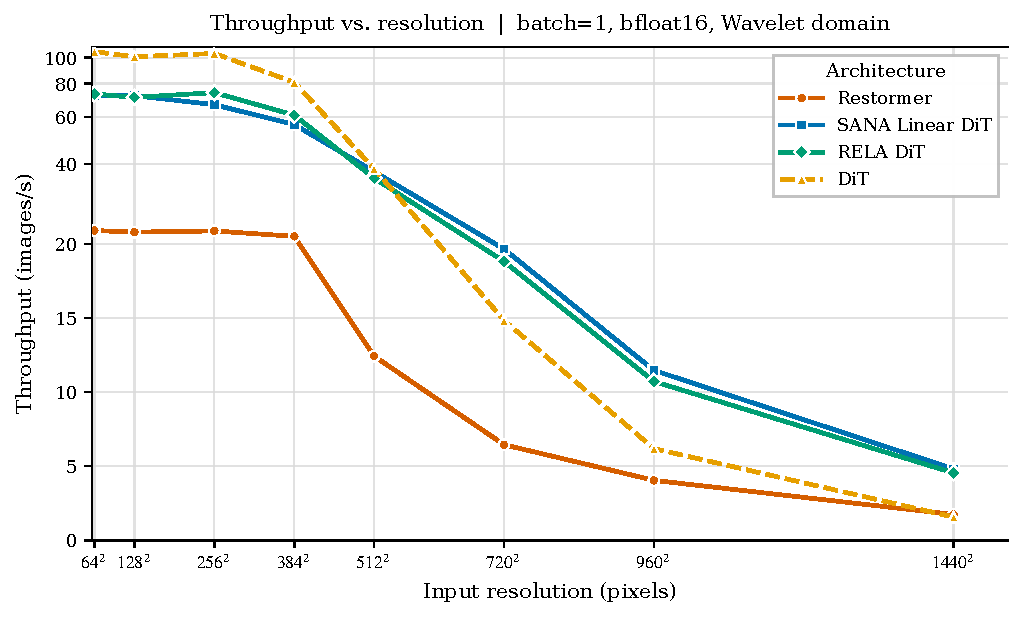
\includegraphics[width=\linewidth]{figures/pdf/throughput_vs_resolution.pdf}
\end{minipage}\hfill
\begin{minipage}[t]{0.42\textwidth}
\centering
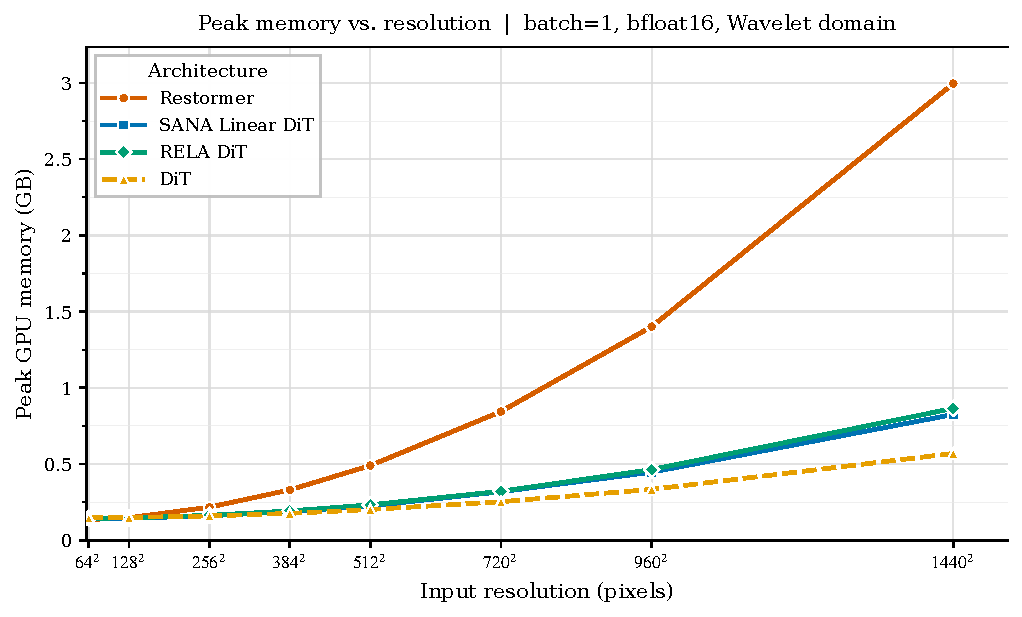
\includegraphics[width=\linewidth]{figures/pdf/memory_vs_resolution.pdf}
\end{minipage}
\captionof{figure}{One-forward-pass scaling in the two-level Haar domain, batch size 1, BF16, RTX 3090. Left: throughput. Right: peak allocated memory. These measurements isolate backbone cost.}
\label{fig:backbone_scaling}
\par\medskip
% Keep the raw measurements on the same page as their plots.
\begin{minipage}{\textwidth}
\centering
\captionof{table}{Eager one-forward-pass architecture benchmark: batch size 1, BF16, two-level Haar, RTX 3090. Resolutions are square.}
\label{tab:backbone_raw}
\scriptsize
\setlength{\tabcolsep}{2pt}
\renewcommand{\arraystretch}{0.85}
\resizebox{\textwidth}{!}{%
\begin{tabular}{r|rrr|rrr|rrr|rrr}
\toprule
&\multicolumn{3}{c|}{Restormer (57.12M)}&\multicolumn{3}{c|}{SANA Linear DiT (64.34M)}&\multicolumn{3}{c|}{RELA DiT (65.32M)}&\multicolumn{3}{c}{DiT (67.47M)}\\
Resolution & ms & img/s & GiB & ms & img/s & GiB & ms & img/s & GiB & ms & img/s & GiB\\
\midrule
$64^2$   &44.4707&22.4867&0.12538&13.8961&71.9626&0.13189&13.6673&73.1673&0.13368&9.4790&105.496&0.13638\\
$128^2$  &45.0920&22.1769&0.13728&13.8650&72.1242&0.13371&14.0712&71.0673&0.13571&9.9097&100.911&0.13871\\
$256^2$  &44.6283&22.4073&0.20189&14.9908&66.7077&0.14912&13.5093&74.0231&0.15194&9.6308&103.834&0.14805\\
$384^2$  &46.7692&21.3816&0.30720&17.8032&56.1697&0.17399&16.4050&60.9571&0.17860&12.356&80.9325&0.16362\\
$512^2$  &80.4425&12.4312&0.45579&26.7253&37.4178&0.20924&28.2868&35.3522&0.21598&26.0815&38.3414&0.18736\\
$720^2$  &155.055&6.4493&0.78590&50.8455&19.6674&0.29607&53.1076&18.8297&0.29880&67.3489&14.8480&0.23488\\
$960^2$  &247.412&4.0418&1.3052&87.1724&11.4715&0.41543&93.2710&10.7214&0.43167&161.674&6.1853&0.31070\\
$1440^2$ &575.833&1.7366&2.7898&207.718&4.8142&0.76812&220.201&4.5413&0.80525&640.170&1.5621&0.53055\\
\bottomrule
\end{tabular}}
\end{minipage}
\end{minipage}
\end{strip}

\subsection{System efficiency}

Table~\ref{tab:system_efficiency} reports 8.05 images/s (0.1242 s) for ours, $2.2\times$ the FBCNN throughput. The SD 2.1 proxy does not establish SODiff deployment speed.

\begin{table}[H]
\centering
\scriptsize
\setlength{\tabcolsep}{3pt}
\renewcommand{\arraystretch}{0.85}
\caption{Reported RTX 3090 batch-one $1024^2$ efficiency. SD 2.1 proxy$^\dagger$ reconstructs the SODiff architecture without its weights; other rows time restoration systems. NFE includes tiles and ensembles.}
\label{tab:system_efficiency}
\resizebox{\columnwidth}{!}{%
\begin{tabular}{lrrrr}
\toprule
Method & \shortstack{Parameters\\(M)} & NFE & \shortstack{Latency\\(s)} & \shortstack{Throughput\\(img/s)}\\
\midrule
FBCNN &70.10&1&0.275&3.63\\
JDEC &38.90&1&0.860&1.16\\
PromptCIR &34.75&64&27.97&0.0358\\
SUPIR &4490&50&48.66&0.0206\\
SD 2.1 proxy$^\dagger$ &1288&1&0.610&1.64\\
\textbf{Ours} &65.32&2&0.1242&8.05\\
\bottomrule
\end{tabular}}
\end{table}

Original RTX 3090 timings are reported aggregates; raw repetitions and the SD 2.1 proxy script are not archived. The 0.610 s proxy follows SODiff's architecture without its weights and does not establish SODiff latency. The released harness uses five warm-ups and 20 synchronized calls, including endpoints/sampling and excluding loading, metrics, and output. Its protocol cannot retroactively define original timing boundaries.

NFE includes tiles/ensembles. Ours uses two full-image calls; FBCNN/JDEC use one. PromptCIR~\cite{li2024promptcir} uses 16 tiles across four checkpoint/transpose passes (64 calls). The Haar/BF16 benchmark separately measures backbone cost.

\subsection{JVP implementation ablation}
\label{sec:jvp_ablation}
Table~\ref{tab:jvp} audits the trained checkpoint on CPU FP32: batch one, $32^2$ synthetic RGB, three noise seeds, identical weights and $(r,t)=(0.2,0.7)$. Primal outputs, tangents, MeanFlow-plus-severity losses, and all parameter gradients agree; LPIPS is excluded. rRMSE denotes relative $L_2$ error. This verifies only these CPU cases. Historical GPU memory reductions are not claimed: their accounting is unrecorded. Audit records and CUDA memory definitions are released.

\begin{table}[H]
\centering
\caption{CPU FP32 JVP audit: trained checkpoint, batch one, $32^2$.}
\label{tab:jvp}
\scriptsize
\setlength{\tabcolsep}{3pt}
\renewcommand{\arraystretch}{0.85}
\begin{tabular}{@{}rrrrr@{}}
\toprule
Seed & Tangent rRMSE & $|\Delta\mathcal L|$ & Gradient rRMSE & Max $|\Delta g|$\\
\midrule
0 &0&0&0&0\\
1 &0&0&0&0\\
2 &0&0&0&0\\
\bottomrule
\end{tabular}
\end{table}

\section{Limitations and Future Work}

Quality uses one seed; no quality ablation isolates Haar, RELA, or severity estimation. Backbone scaling measures cost, not quality attribution. The 13,450-image training pool may limit semantic knowledge; generated detail need not recover missing information faithfully. Larger-scale training may help. Method-specific precision, tiling, and sampling limit speed comparisons.

\section{Conclusion}

Haar-domain residuals and a RELA DiT enable two-update MeanFlow restoration without a VAE or pretrained generator. Our 65.32M-parameter model reaches 8.05 images/s at $1024^2$ with competitive LPIPS. Larger pretrained priors retain advantages under severe compression and on other metrics.

\section*{Acknowledgments}
We thank Radu Miron and Andrei Ciortea for their valuable feedback and helpful discussions. % This work is not officially supervised, funded, or endorsed by ...

\bibliography{main}

% Keep the single qualitative appendix together below the references.
\setlength{\stripsep}{4pt}
\begin{strip}
\begin{minipage}{\textwidth}
\appendix[Qualitative Results]
\label{app:qualitative}
Illustrative $512\times512$ LSDIR crops: left, QF 10/two updates; right, QF 5/one update.
\par
\centering
\setlength{\tabcolsep}{1.5pt}
\newcommand{\qualimg}[1]{\includegraphics[width=0.085\textwidth]{#1}}
\begin{tabular}{@{}ccc@{\hspace{7pt}}ccc@{}}
\textbf{JPEG} & \textbf{Ours} & \textbf{Reference} &
\textbf{JPEG} & \textbf{Ours} & \textbf{Reference}\\
\qualimg{figures/qualitative_crops/appendix_05_qf10.png} &
\qualimg{figures/qualitative_crops/appendix_05_qf10_s2.png} &
\qualimg{figures/qualitative_crops/appendix_05_ref.png} &
\qualimg{figures/qualitative_crops/appendix_08_qf5.png} &
\qualimg{figures/qualitative_crops/appendix_08_qf5_s1.png} &
\qualimg{figures/qualitative_crops/appendix_08_ref.png}\\[-2pt]
\multicolumn{3}{c}{\scriptsize QF 10, 2 steps} & \multicolumn{3}{c}{\scriptsize QF 5, 1 step}
\end{tabular}
\end{minipage}
\end{strip}

\end{document}
